% =====================================================================================
% CERTA -- Figure 1 (architecture). Standalone; compiles in Overleaf to fig1.pdf.
% Engine: pdfLaTeX. Output crops tight to the diagram (standalone `border`).
% To place it in the manuscript, compile this file and \includegraphics{fig1.pdf},
% OR paste the \begin{tikzpicture}...\end{tikzpicture} block into your figure
% environment and move the \definecolor / \usetikzlibrary lines into your preamble.
% =====================================================================================
\documentclass[border=8pt]{standalone}
\usepackage{amssymb}
\usepackage{tikz}
\usetikzlibrary{arrows.meta,positioning,calc,backgrounds}

% ---- Tailwind-style palette used by the node styles ---------------------------------
\definecolor{slate50}{HTML}{F8FAFC}
\definecolor{slate300}{HTML}{CBD5E1}
\definecolor{slate600}{HTML}{475569}
\definecolor{slate800}{HTML}{1E293B}
\definecolor{amber50}{HTML}{FFFBEB}
\definecolor{amber700}{HTML}{B45309}
\definecolor{emerald50}{HTML}{ECFDF5}
\definecolor{emerald700}{HTML}{047857}
\definecolor{rose50}{HTML}{FFF1F2}
\definecolor{rose700}{HTML}{BE123C}

\begin{document}
\hyphenpenalty=10000 \exhyphenpenalty=10000
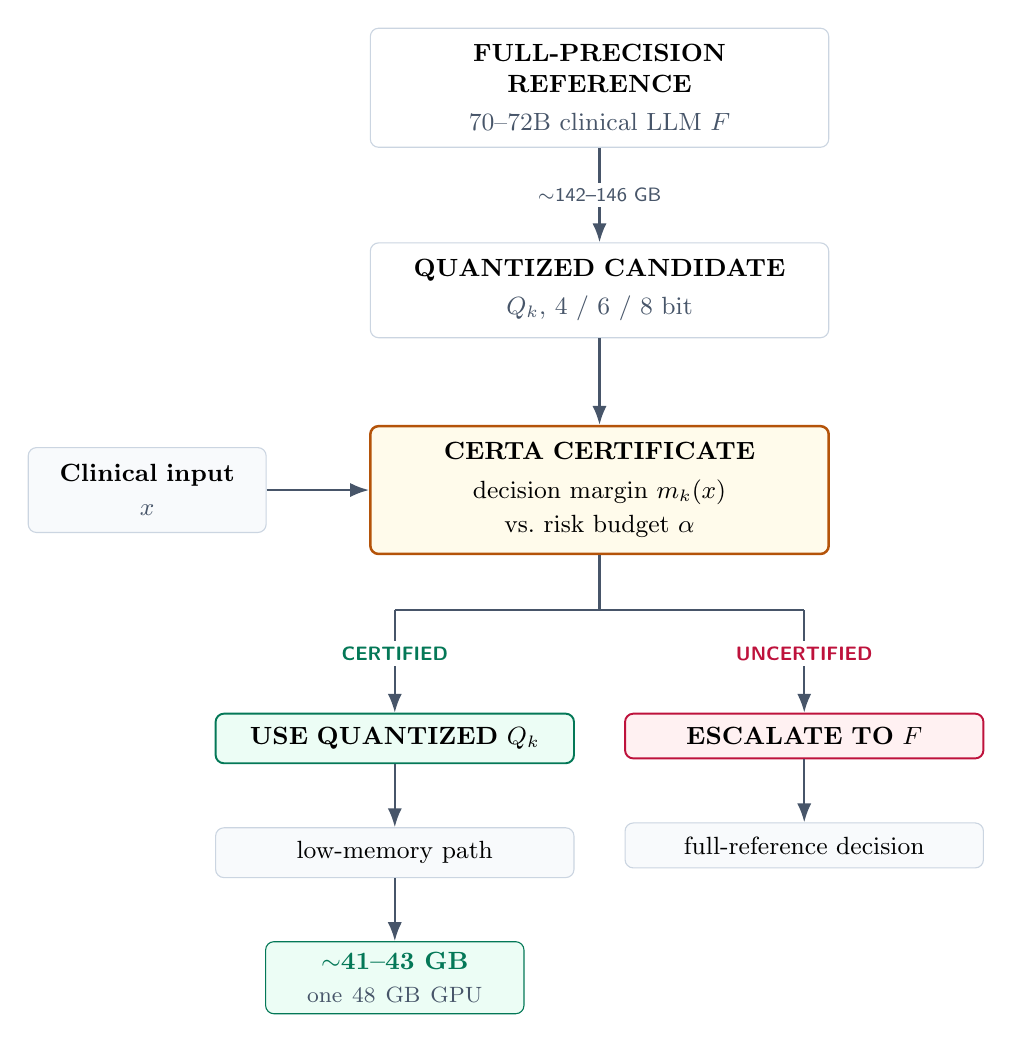
\begin{tikzpicture}[
  font=\sffamily,
  >=Latex,
  card/.style={
    draw=slate300, fill=white, rounded corners=3pt, align=center,
    text width=54mm, inner sep=6pt, font=\small},
  certaBox/.style={
    draw=amber700, fill=amber50, rounded corners=3pt, align=center,
    text width=54mm, inner sep=6pt, line width=0.9pt, font=\small},
  useBox/.style={
    draw=emerald700, fill=emerald50, rounded corners=3pt, align=center,
    text width=42mm, inner sep=5pt, font=\small, line width=0.7pt},
  escBox/.style={
    draw=rose700, fill=rose50, rounded corners=3pt, align=center,
    text width=42mm, inner sep=5pt, font=\small, line width=0.7pt},
  subCard/.style={
    draw=slate300, fill=slate50, rounded corners=3pt, align=center,
    text width=42mm, inner sep=5pt, font=\small},
  vramBadge/.style={
    draw=emerald700, fill=emerald50, rounded corners=3pt, align=center,
    text width=30mm, inner sep=4pt, font=\small\bfseries, text=emerald700},
  arr/.style={-{Latex[length=2.4mm]}, line width=0.8pt, color=slate600},
  line/.style={line width=0.8pt, color=slate600},
  lbl/.style={font=\scriptsize\sffamily, text=slate600, fill=white, inner sep=2pt},
  brlbl/.style={font=\scriptsize\sffamily\bfseries, fill=white, inner sep=2pt}
]
  % 1. Full-precision reference
  \node[card] (ref) {\textbf{FULL-PRECISION REFERENCE}\\[1mm]
    \textcolor{slate600}{70--72B clinical LLM $F$}};
  % 2. Quantized candidate
  \node[card, below=12mm of ref] (quant) {\textbf{QUANTIZED CANDIDATE}\\[1mm]
    \textcolor{slate600}{$Q_k$, 4 / 6 / 8 bit}};
  \draw[arr] (ref) -- node[lbl] {$\sim$142--146 GB} (quant);
  % 3. CERTA
  \node[certaBox, below=11mm of quant] (certa) {\textbf{CERTA CERTIFICATE}\\[1mm]
    decision margin $m_k(x)$\\[0.5mm] vs.\ risk budget $\alpha$};
  \draw[arr] (quant) -- (certa);
  % Side input
  \node[card, left=13mm of certa, text width=26mm, fill=slate50] (input)
    {\textbf{Clinical input}\\[0.5mm]\textcolor{slate600}{$x$}};
  \draw[arr] (input) -- (certa);
  % Fork
  \coordinate (fork)      at ($(certa.south) + (0,-7mm)$);
  \coordinate (forkLeft)  at ($(fork) + (-26mm,0)$);
  \coordinate (forkRight) at ($(fork) + ( 26mm,0)$);
  \draw[line] (certa.south) -- (fork);
  \draw[line] (forkLeft) -- (forkRight);
  % 4. Certified branch (left)
  \node[useBox, below=13mm of forkLeft] (use) {\textbf{USE QUANTIZED $Q_k$}};
  \draw[arr] (forkLeft) -- node[brlbl, text=emerald700, pos=0.42] {CERTIFIED} (use);
  % 5. Escalate branch (right)
  \node[escBox, below=13mm of forkRight] (esc) {\textbf{ESCALATE TO $F$}};
  \draw[arr] (forkRight) -- node[brlbl, text=rose700, pos=0.42] {UNCERTIFIED} (esc);
  % 6. Destinations
  \node[subCard, below=8mm of use]  (lowmem)  {low-memory path};
  \draw[arr] (use) -- (lowmem);
  \node[subCard, below=8mm of esc]  (fullref) {full-reference decision};
  \draw[arr] (esc) -- (fullref);
  % 7. Final VRAM target
  \node[vramBadge, below=8mm of lowmem] (vramEnd) {$\sim$41--43 GB\\[0.3mm]
    \textcolor{slate600}{\footnotesize\mdseries one 48 GB GPU}};
  \draw[arr] (lowmem) -- (vramEnd);
\end{tikzpicture}
\end{document}
